\documentclass{beamer}
\usetheme{metropolis}

\metroset{progressbar=frametitle, titleformat=smallcaps, block=fill}
\makeatletter
\setlength{\metropolis@titleseparator@linewidth}{1pt}
\setlength{\metropolis@progressonsectionpage@linewidth}{1.5pt}
\setlength{\metropolis@progressinheadfoot@linewidth}{2pt}
\makeatother

\usepackage{float}
\usepackage{tikz}
\usetikzlibrary{positioning}
\usetikzlibrary{arrows.meta}
\usetikzlibrary{calc}
\tikzset{>=Latex}

\title{Deep Checker}
\subtitle{Apprentissage statistique et intelligence artificielle}
\date{}
\author{Arthur Correnson, Igor Martayan, Manon Sourisseau}
\titlegraphic{\hfill
\includegraphics[height=1.5cm]{im/logo.pdf}}
\institute{Projet de Statistiques, ENS, 2021}

\begin{document}

{\metroset{background=dark}\maketitle}

\begin{frame}{Introduction}
    \begin{columns}
        \column{0.6\textwidth}
        \begin{itemize}
            \item Construction d'une \alert{heuristique} évaluant la qualité des coups
            \item 3 problématiques :
                  \begin{itemize}
                      \item Génération des données
                      \item Choix des modèles
                      \item Mise en place des modèles
                  \end{itemize}
        \end{itemize}
        \column{0.4\textwidth}
        \begin{figure}
            \centering
            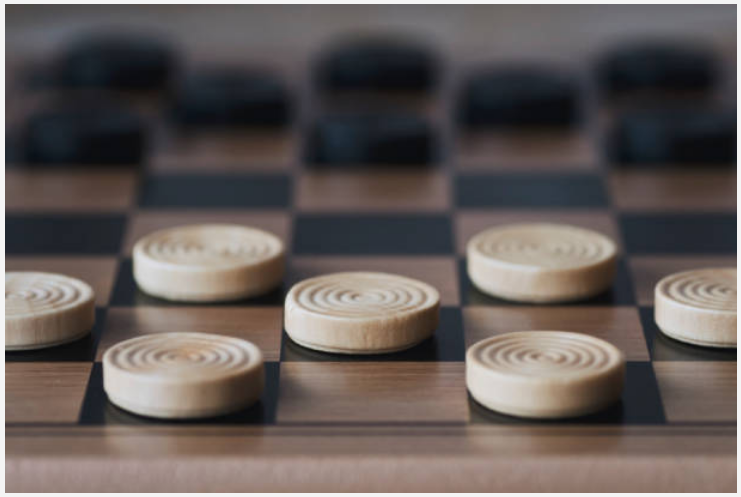
\includegraphics[width=\columnwidth]{im/dames.png}
        \end{figure}
    \end{columns}
\end{frame}

\begin{frame}{Plan de la présentation}
    \setbeamertemplate{section in toc}[sections numbered]
    \tableofcontents
\end{frame}

{\metroset{background=dark}\section{Génération de données et simulateur}}

\begin{frame}{Génération de données}
    \begin{itemize}
        \item Besoin d'un \alert{grand nombre de données}
        \item Générer beaucoup de parties \alert{rapidement} et de manière \alert{compacte} en mémoire
        \item Écriture d'un simulateur dans le langage \alert{C}
    \end{itemize}
\end{frame}

\begin{frame}{Création d'un simulateur}
    \begin{columns}
        \column{0.6\textwidth}
        \begin{itemize}
            \item 64 cases, 32 cases possibles
            \item 3 états possibles par cases : \newline
                  Vide, pion blanc, pion noir
        \end{itemize}
        Représentation de l'état du plateau par un entier de 64 bits (\alert{2 x 32 bits})
        exemple : 1111 1111 1111 0000 0000 0000 0000 0000 // 0000 0000 0000 0000 0000 1111 1111 1111

        \column{0.4\textwidth}
        \begin{figure}
            \centering
            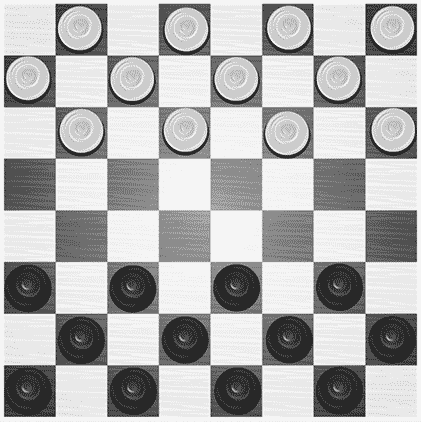
\includegraphics[width=\columnwidth]{im/dames2.png}
        \end{figure}
    \end{columns}
\end{frame}

\begin{frame}[fragile]{Données et performances}
    \begin{itemize}
        \item Les données sont stockées dans un fichier texte. \newline
              (perte d'efficacité contre simplicité de traitement des données)
        \item Performances très satisfaisantes : \newline
              \alert{10 000} parties générées en environ \alert{1 secondes}, sur un ordinateur ordinaire.
    \end{itemize}
    \begin{verbatim}
unsigned do_move_left(unsigned pos,
    unsigned *player, int direction) {
  unsigned pos_next = next_left(pos, direction);
  *player ^= (1 << pos) | (1 << pos_next);
  return pos_next;
}
    \end{verbatim}
\end{frame}

{\metroset{background=dark}\section{Modèles et heuristiques}}

\begin{frame}{Modèles et heuristiques}
    On souhaite construire une heuristique qui attribue un \alert{score} à un coup donné, selon la \alert{qualité} du coup.
    Plusieurs approches pour déterminer l'heuristique :
    \begin{itemize}
        \item Régression par les K plus proches voisins (KNN)
        \item Réseau de neurones type perceptron multicouche (MLP)
    \end{itemize}
    Le but est de jouer le coup possible ayant le meilleur score.
\end{frame}

\begin{frame}{Modélisation du problème}
    Étant donné un ensemble $\mathcal{DB}$ de parties simulées,
    on souhaite donner une première approximation de l'heuristique $h$.
    \begin{itemize}
        \item On introduit une fonction d'évaluation $\lVert.\rVert_i : C_i \to [-1, 1]$
              définie comme $\lVert c \rVert_i = \frac{1}{\sqrt{d(c)}}.v(c)$
              \begin{itemize}
                  \item $C_i$ l'ensemble des coups dans une partie $P_i \in \mathcal{DB}$
                  \item $d(c) \in \mathbb{N}$ le nombre de coups qui séparent $c$ de la fin de partie
                  \item $v(c) = 1$ ou $v(c) = -1$ selon que la partie est gagnée ou perdue
              \end{itemize}
        \item Le score final d'un coup $c$ est la moyenne des scores qui lui sont attribués sur l'ensemble des parties dans $\mathcal{DB}$
    \end{itemize}
\end{frame}

{\metroset{background=dark}\section{Régression aux k plus proches voisins}}

\begin{frame}{Régression par KNN}
    KNN : méthode de régression aux \alert{K plus proche voisins}.
    On définit la distance entre deux coups par la \alert{distance d'édition} :
    $$ \langle c_1, c_2 \rangle_{KNN} = \ \rVert c_1 \oplus c_2 \lVert_1 $$
    $\rightarrow$ Les coups sont représentés comme des entiers de 128 bits.
    \begin{itemize}
        \item On calcule la distance du coup donné avec tous les autres coups.
        \item Le score attribué au coup donné correspond à \alert{la moyenne des scores} des K plus proches voisins.
    \end{itemize}
\end{frame}

\begin{frame}{Résultat et performances de KNN}
    \begin{center}
        \begin{tabular}{ | c | c | }
            \hline
            Victoires du joueur 1 (KNN) & Victoires du joueur 2 (Aléatoire) \\ \hline
            18                          & 32                                \\ \hline
        \end{tabular}
    \end{center}
    Cette version de l'heuristique est peu satisfaisante :
    \begin{itemize}
        \item La notation d'un coup met l'accent sur les variations très \textbf{locales}
        \item La distance choisie rapproche uniquement les coups qui se ressemble en terme d'état \textbf{global} du jeu
    \end{itemize}
\end{frame}

{\metroset{background=dark}\section{Amélioration de l'heuristique}}

\begin{frame}{Nouveau calcul de score}
    \begin{itemize}
        \item Nouvelle fonction d'évaluation : \newline
              $\lVert.\rVert_i : D_i \to \mathbb{N}$ définie comme : $\lVert d \rVert_i = p(d).v(d)$
              \begin{itemize}
                  \item $D_i$ : Ensemble des états du damier vu par le joueur 1
                  \item $p(d) \in \mathbb{N}$ : Nombre de pions mangé depuis l'état $d$
                  \item  $v(d) = 1$ si le joueur 1 gagne, $v(d) = 0$ sinon
              \end{itemize}
        \item On construit maintenant une fonction $w_i(c)$ telle que $w_i(d) = \lVert c \lVert_i$ si $d \in D_i$ et $w_i(d) = 0$ sinon
        \item Pour chaque état de damier $d$ apparaissant dans l'ensemble des parties de $\mathcal{DB}$, $h(d) = \frac{1}{N}\Sigma w_i(d)$ avec $N$ le nombre de parties $P_i$ tels que $w_i(d) \neq 0$ ($d$ est l'un des états pris par le damier dans $P_i$)
    \end{itemize}
\end{frame}

\begin{frame}{Nouveaux résultats de KNN}
    \begin{center}
        \begin{tabular}{ | c | c | }
            \hline
            Victoires du joueur 1 (KNN) & Victoires du joueur 2 (Aléatoire) \\ \hline
            34                          & 16                                \\ \hline
        \end{tabular}
    \end{center}
    Cette version de l'heuristique est plus satisfaisante. \newline
    Le temps de calcul reste toutefois assez élevé.
\end{frame}

{\metroset{background=dark}\section{Perceptron multicouche}}

\begin{frame}{Crash course sur les réseaux de neurones}
    \begin{figure}
        \begin{tikzpicture}[node distance=1.5cm and 1.5cm]
            \node[circle, draw] (X1) {$x_1$};
            \node[circle, draw] (X2) [below=of X1] {$x_2$};
            \node[circle, draw] (S1) [right=of X1] {$s_1$};
            \node[circle, draw] (S2) [right=of X2] {$s_2$};
            \node[circle, draw] (X1') [right=of S1] {$x_1$'};
            \node[circle, draw] (X2') [right=of S2] {$x_2$'};
            \node (M) at ($(X1') !.5! (X2')$) {};
            \node[circle, draw] (S') [right=of M] {$s'$};
            \node[circle, draw] (Y) [right=of S'] {$y$};
            \path[->]
            (X1) edge (S1) edge (S2)
            (X2) edge (S1) edge (S2)
            (S1) edge node[above] {$\sigma$} (X1')
            (S2) edge node[above] {$\sigma$} (X2')
            (X1') edge (S')
            (X2') edge (S')
            (S') edge node[above] {$\sigma$} (Y);
        \end{tikzpicture}
        \caption{Perceptron avec une couche cachée}
    \end{figure}
    \begin{itemize}
        \item propagation : $s = W.x + b$, $x' = \sigma(s)$
        \item descente de gradient : $W \leftarrow W - \alpha \frac{\partial \Delta}{\partial W}$
    \end{itemize}
\end{frame}

\begin{frame}{Perceptron multicouche (MLP)}
    \begin{itemize}
        \item Entrées : vecteurs de 64 bits (représentant un unique damier)
        \item Coeur du réseau : 4 couches intermédiaires (64, 64, 32, 16)
        \item Noeuds du réseau : fonction d'activation \alert{relu}
        \item Sortie du réseau de dimension 1 (régression) : combinaison linéraire des 16 sorties de la dernière couche puis d'une application de \alert{relu}
    \end{itemize}
\end{frame}

\begin{frame}{Résultats du perceptron multicouche}
    \begin{center}
        \begin{tabular}{ | c | c | }
            \hline
            Victoires du joueur 1 (MLP) & Victoires du joueur 2 (Aléatoire) \\ \hline
            50                          & 0                                 \\ \hline
        \end{tabular}
    \end{center}
    $\rightarrow$ Heuristique bien plus satisfaisante, temps de calcul plus rapide
\end{frame}

\begin{frame}{Coefficient de détermination}
    $$R^2 = 1 - \sum_{i=1}^{n} \frac{(y_i - \hat{y_i})^2}{(y_i - \bar{y})^2}$$
    \begin{center}
        \begin{tabular}{ | l | c | }
            \hline
            Heuristique            & $R^2$ \\ \hline
            Distance à la victoire & 0.46  \\ \hline
            Nombre de prises       & 0.68  \\ \hline
        \end{tabular}
    \end{center}
\end{frame}

\begin{frame}{Résultats finaux}
    \begin{center}
        \begin{tabular}{ | c || c | c |}
            \hline
            Heuristiques + Models        & Victoires & Défaites \\
            \hline
            \hline
            Distance à la victoire + KNN & 18        & 32       \\
            Nombre de prises + KNN       & 36        & 14       \\
            Distance à la victoire + MLP & 39        & 11       \\
            Nombre de prises + MLP       & 50        & 0        \\ \hline
        \end{tabular}

    \end{center}
\end{frame}


{\metroset{background=dark}\section*{Conclusion}}

\begin{frame}{Conclusion}
    Pistes d'amélioration :
    \begin{itemize}
        \item Heuristiques plus fines
        \item Techniques d'apprentissage par renforcement
        \item Réseaux de neurones convolutifs
        \item Arbre de Monte-Carlo
    \end{itemize}
\end{frame}

\appendix

{\metroset{background=dark}\section*{Questions ?}}

\begin{frame}{Références}
    \begin{enumerate}
        \item Multi Layer Perceptron, \url{https://en.wikipedia.org/wiki/Multilayer_perceptron}, Wikipédia

        \item K-nearest nieghbors algorithm, \url{https://en.wikipedia.org/wiki/K-nearest_neighbors_algorithm}, Wikipédia

        \item Scikit-learn: Machine Learning in Python \url{https://scikit-learn.org/stable/} Pedregosa et al., \textbf{Journal of Machine Learning Research}, 2012

        \item Levenshtein distance, \url{https://en.wikipedia.org/wiki/Levenshtein_distance}, Wikipédia

        \item Coefficient of determination, \url{https://en.wikipedia.org/wiki/Coefficient_of_determination}, Wikipédia
    \end{enumerate}
\end{frame}

\end{document}
